\documentclass[usenames,dvipsnames,tikz]{standalone}
%\usepackage{amsmath,amssymb}
%\usepackage{xcolor}
\colorlet{tBlue}{RoyalBlue!35!Cerulean}
\colorlet{tRed}{Red}
%\usepackage{tikz}
%\usepackage{standalone}
\begin{document}
	
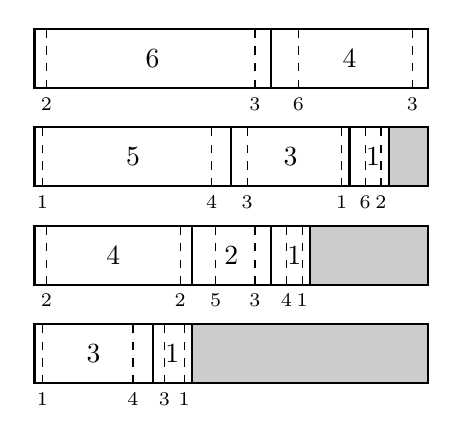
\begin{tikzpicture}
%\draw [help lines] (-1,-2) grid (13,5);
% 1=0.1, 2=0.15, 3=0.2, 4=0.25, 5=0.3
% 6, 5, 4, 4, 3, 3, 2, 1, 1, 1.

%---------------------------------------------------------------------
% SCPP
% 1=0.1, 2=0.15, 3=0.2, 4=0.25, 5=0.3
\draw [thick] (0,0) rectangle (5,0.75);
\draw [thick] (0,1.25) rectangle (5,2);
\draw [thick] (0,2.5) rectangle (5,3.25);
\draw [thick] (0,3.75) rectangle (5,4.5);

% Bottom row, 3, 1 (1-4, 3-1, sixth, tenth)
\draw [thick] (1.5,0) -- (1.5,0.75);
\draw [thick] (2,0) -- (2,0.75);
\filldraw[fill=black!20!white, draw=black, thick] (2,0) rectangle (5,0.75);
\draw [dashed] (0.1,0) -- (0.1,0.75);
\draw [dashed] (1.25,0) -- (1.25,0.75);
\draw [dashed] (1.65,0) -- (1.65,0.75);
\draw [dashed] (1.9,0) -- (1.9,0.75);
\node [below] at (0.1,0) {\scriptsize{1}};
\node [below] at (1.25,0) {\scriptsize{4}};
\node [below] at (1.65,0) {\scriptsize{3}};
\node [below] at (1.9,0) {\scriptsize{1}};
\node at (0.75,0.375) {3};
\node at (1.75,0.375) {1};

% Second from bottom row, 4, 2, 1 (2-2, 5-3, 4-1, fourth, seventh, ninth)
\draw [thick] (2,1.25) -- (2,2);
\draw [thick] (3,1.25) -- (3,2);
\draw [thick] (3.5,1.25) -- (3.5,2);
\filldraw[fill=black!20!white, draw=black, thick] (3.5,1.25) rectangle (5,2);
\draw [dashed] (0.15,1.25) -- (0.15,2);
\draw [dashed] (1.85,1.25) -- (1.85,2);
\draw [dashed] (2.3,1.25) -- (2.3,2);
\draw [dashed] (2.8,1.25) -- (2.8,2);
\draw [dashed] (3.2,1.25) -- (3.2,2);
\draw [dashed] (3.4,1.25) -- (3.4,2);
\node [below] at (0.15,1.25) {\scriptsize{2}};
\node [below] at (1.85,1.25) {\scriptsize{2}};
\node [below] at (2.3,1.25) {\scriptsize{5}};
\node [below] at (2.8,1.25) {\scriptsize{3}};
\node [below] at (3.2,1.25) {\scriptsize{4}};
\node [below] at (3.4,1.25) {\scriptsize{1}};
\node at (1,1.625) {4};
\node at (2.5,1.625) {2};
\node at (3.3,1.625) {1};

% Second from top row, 5, 3, 1 (1-4, 3-1, 6-2, second, fifth, eighth)
\draw [thick] (2.5,2.5) -- (2.5,3.25);
\draw [thick] (4,2.5) -- (4,3.25);
\draw [thick] (4.5,2.5) -- (4.5, 3.25);
\filldraw[fill=black!20!white, draw=black, thick] (4.5,2.5) rectangle (5,3.25);
\draw [dashed] (0.1,2.5) -- (0.1,3.25);
\draw [dashed] (2.25,2.5) -- (2.25,3.25);
\draw [dashed] (2.7,2.5) -- (2.7,3.25);
\draw [dashed] (3.9,2.5) -- (3.9,3.25);
\draw [dashed] (4.2,2.5) -- (4.2,3.25);
\draw [dashed] (4.4,2.5) -- (4.4,3.25);
\node [below] at (0.1,2.5) {\scriptsize{1}};
\node [below] at (2.25,2.5) {\scriptsize{4}};
\node [below] at (2.7,2.5) {\scriptsize{3}};
\node [below] at (3.9,2.5) {\scriptsize{1}};
\node [below] at (4.2,2.5) {\scriptsize{6}};
\node [below] at (4.4,2.5) {\scriptsize{2}};
\node at (1.25,2.875) {5};
\node at (3.25,2.875) {3};
\node at (4.3,2.875) {1};

% Top row, 6,4 (2-3, 6-3, first, third)
\draw [thick] (3,3.75) -- (3,4.5);
\draw [dashed] (0.15,3.75) -- (0.15,4.5);
\draw [dashed] (2.8,3.75) -- (2.8,4.5);
\draw [dashed] (3.35,3.75) -- (3.35,4.5);
\draw [dashed] (4.8,3.75) -- (4.8,4.5);
\node [below] at (0.15,3.75) {\scriptsize{2}};
\node [below] at (2.8,3.75) {\scriptsize{3}};
\node [below] at (3.35,3.75) {\scriptsize{6}};
\node [below] at (4.8,3.75) {\scriptsize{3}};
\node at (1.5,4.125) {6};
\node at (4,4.125) {4};

\end{tikzpicture}

\end{document}